\section{Introduction}\raggedbottom 

QANet is a state of the art neural network for solving the question answering problem with a single which does not use any recurrent neural nets(RNN) as most of the other state of the art approaches. As RNNs take a lot of time to train this is a advantage in performance. I am trying to use this new architecture in a chatbot where state of the art models use RNNs to see what performance improvement is reached by this.

\begin{figure}[htb]
\begin{center}
  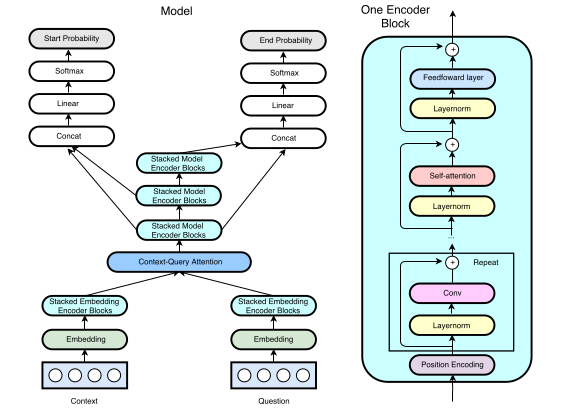
\includegraphics[width=300pt, angle=0]{bilder/QANetArchitecture}
  \caption{An overview of the QANet architecture}\label{fig_QANet}
\end{center}
\end{figure}


\pagebreak
\section{Weiteres Kapitel}\raggedbottom 
\subsection{Unterkapitel}
\subsection{Unterkapitel}